% Provenance (never printed): cycle 2 "Questionner le monde de la matiere"
% (solid materials, observing and sorting) and cycle 3 theme 4 (local geology,
% rocks for building); see sources/book1/PROVENANCE.md. Book 1, grade 3, ch. 1.
\chapter{Piedras, cantos rodados y arena}\label{ch:g3:stones-pebbles-sand}

Tom está de vacaciones junto a un \omterm{def:g1:landscapes-around-us:water}{río}. En la orilla de \omterm{def:g3:stones-pebbles-sand:pebble}{grava}, donde el agua
es poco profunda, recoge un \omterm{def:g3:stones-pebbles-sand:pebble}{canto}. Es liso y redondo, casi como un huevo, y
le cabe en la mano. La semana pasada, paseando con sus padres por un
sendero de \omterm{def:g1:landscapes-around-us:landform}{montaña}, mucho más arriba en el mismo \omterm{def:g1:landscapes-around-us:landform}{valle}, vio piedras del
mismo color tiradas al pie de una ladera rocosa --- pero aquellas piedras
eran afiladas, con aristas y esquinas.

¿Cómo se convirtió una piedra afilada de la \omterm{def:g1:landscapes-around-us:landform}{montaña} en un \omterm{def:g3:stones-pebbles-sand:pebble}{canto} liso y
redondo en el fondo del \omterm{def:g1:landscapes-around-us:landform}{valle}? Para averiguarlo, empecemos por la propia
\omterm{def:g3:stones-pebbles-sand:rock}{roca}.

\begin{omfigure}
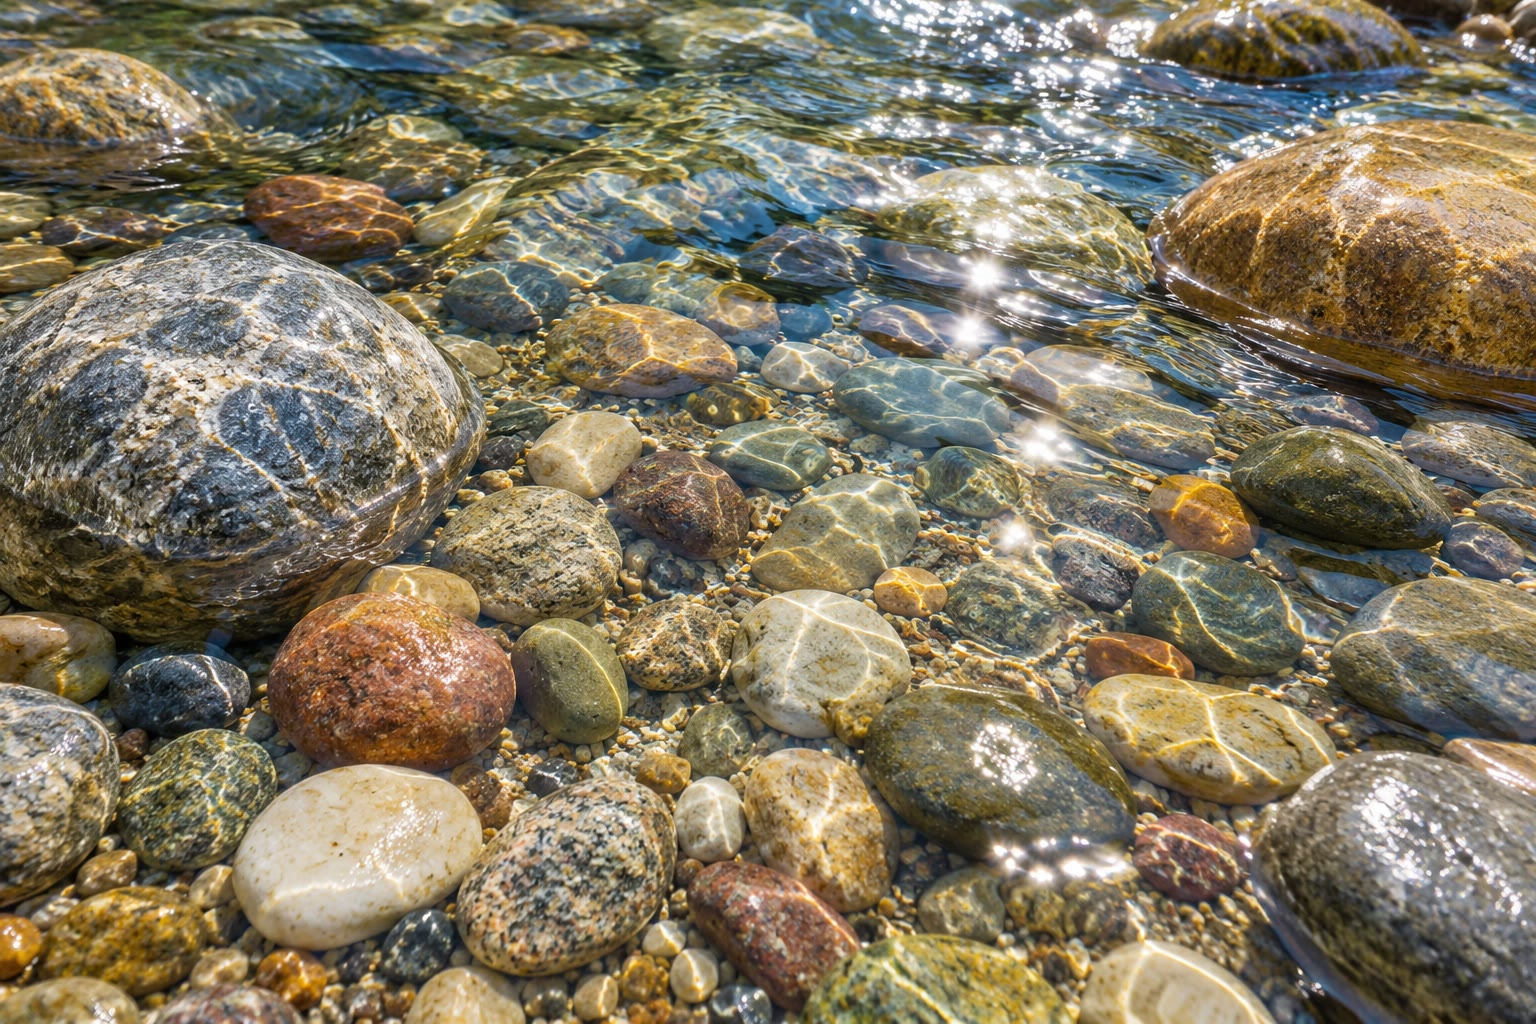
\includegraphics[width=0.62\linewidth]{images/book1/ai/g3-stream-pebbles.jpg}

{\small \omterm{def:g3:stones-pebbles-sand:pebble}{Cantos} redondos bajo el agua clara de un arroyo.}
\end{omfigure}

\begin{recall}
En un \omterm{def:g1:landscapes-around-us:landscape}{paisaje} hay \omterm{def:g1:landscapes-around-us:landform}{montañas}, \omterm{def:g1:landscapes-around-us:landform}{colinas}, \omterm{def:g1:landscapes-around-us:landform}{valles} y \omterm{def:g1:landscapes-around-us:landform}{llanuras}, y \omterm{def:g1:landscapes-around-us:water}{ríos} que bajan
de las tierras altas hasta el \omterm{def:g2:water-on-earth:ocean}{mar} (\cref{ch:g1:landscapes-around-us}). La
capa de arriba del terreno, donde crecen las plantas, es el suelo: los
libros de biología cuentan cómo lo fabrican los seres vivos.
\end{recall}

\section{La roca: el suelo duro bajo nuestros pies}

Cava un hoyo profundo en un jardín. Primero encuentras una tierra oscura y
blanda, con raíces. Más abajo, la tierra se vuelve más clara y más
pedregosa. Y si pudieras cavar lo bastante hondo, siempre llegarías a algo
duro que una pala no puede cortar: la \omterm{def:g3:stones-pebbles-sand:rock}{roca}.

\begin{definition}[Roca y lecho rocoso]\label{def:g3:stones-pebbles-sand:rock}
Una \emph{roca}\index{roca} es un material duro y natural del que está hecha
la Tierra sólida. El \emph{lecho rocoso}\index{lecho rocoso} es la roca
sólida que hay bajo el suelo en todas partes en tierra firme, y bajo la
\omterm{def:g3:stones-pebbles-sand:sand}{arena} y el \omterm{def:g3:stones-pebbles-sand:sand}{barro} del fondo del \omterm{def:g2:water-on-earth:ocean}{mar}.
\end{definition}

En la mayoría de los lugares el \omterm{def:g3:stones-pebbles-sand:rock}{lecho rocoso} está escondido bajo el suelo,
la hierba y los árboles. Lo vemos donde no hay suelo que lo cubra: en las
laderas empinadas de las \omterm{def:g1:landscapes-around-us:landform}{montañas}, en los acantilados junto al \omterm{def:g2:water-on-earth:ocean}{mar} y a lo
largo de las carreteras que se han abierto a través de una \omterm{def:g1:landscapes-around-us:landform}{colina}.

\begin{omfigure}
\begin{tikzpicture}[x=1cm, y=1cm, font=\small]
  % bedrock
  \fill[omLithGranite!60] (0,0) rectangle (11,2.2);
  \foreach \x/\y in {0.6/0.5, 1.8/1.4, 3.1/0.7, 4.4/1.6, 5.6/0.4, 6.9/1.2, 8.3/0.6, 9.6/1.5, 10.3/0.4}
    \draw[black!40, line width=0.4pt] (\x,\y) -- ++(0.5,0.25);
  % soil (thick on the left, missing on the steep right)
  \fill[brown!55] (0,2.2) -- (0,3.4) .. controls (2,3.5) and (4,3.4) .. (5.6,3.2) -- (6.4,2.9) -- (6.4,2.2) -- cycle;
  \fill[brown!30] (0,2.2) rectangle (6.4,2.65);
  % rock showing on the right: a hill side with no soil
  \fill[omLithGranite!60] (6.4,2.2) -- (6.4,2.9) -- (7.6,3.9) -- (8.8,4.3) -- (11,4.3) -- (11,2.2) -- cycle;
  \draw[black!60] (0,3.4) .. controls (2,3.5) and (4,3.4) .. (5.6,3.2) -- (6.4,2.9) -- (7.6,3.9) -- (8.8,4.3) -- (11,4.3);
  % grass and roots
  \foreach \x in {0.3,0.8,...,5.3}
    \draw[green!50!black, line width=0.6pt] (\x,{3.4-0.04*\x}) -- ++(0.05,0.18);
  \foreach \x in {1.2,3.4,4.9}
    \draw[brown!80!black, line width=0.5pt] (\x,3.3) -- ++(-0.1,-0.5) -- ++(0.15,-0.3);
  % labels
  \node[anchor=west] at (11.2,3.6) {roca que se ve};
  \node[anchor=west] at (11.2,3.2) {en la superficie};
  \draw[black!60] (11.15,3.4) -- (9.6,4.15);
  \node[anchor=east] at (-0.2,2.9) {suelo};
  \draw[black!60] (-0.15,2.9) -- (0.6,2.9);
  \node[anchor=west] at (11.2,1.1) {lecho rocoso};
  \draw[black!60] (11.15,1.1) -- (10.6,1.1);
\end{tikzpicture}

{\small Un corte del terreno. Bajo el suelo siempre está el \omterm{def:g3:stones-pebbles-sand:rock}{lecho rocoso}
sólido. En la ladera empinada, a la derecha, falta el suelo y la \omterm{def:g3:stones-pebbles-sand:rock}{roca}
aparece en la superficie.}
\label{fig:g3:stones-pebbles-sand:ground}
\end{omfigure}

\section{De la roca a los cantos rodados}

La \omterm{def:g3:stones-pebbles-sand:rock}{roca} es dura, pero no dura para siempre. En invierno, el agua se mete en
las grietas de una \omterm{def:g3:stones-pebbles-sand:rock}{roca}, se congela, se hincha y ensancha las grietas. Las
raíces también crecen dentro de las grietas. Poco a poco se desprenden
trozos que caen: de ahí vienen las piedras afiladas que hay al pie de las
laderas de las \omterm{def:g1:landscapes-around-us:landform}{montañas}.

Cuando una piedra afilada cae a un arroyo de \omterm{def:g1:landscapes-around-us:landform}{montaña}, el agua la hace rodar
por el fondo, la golpea contra otras piedras y la arrastra sobre la \omterm{def:g3:stones-pebbles-sand:sand}{arena}.
Sus esquinas son lo primero que se gasta. Cuanto más lejos viaja, más
redonda y lisa se vuelve. Cuando llega a la parte baja del \omterm{def:g1:landscapes-around-us:landform}{valle}, se ha
convertido en un \omterm{def:g3:stones-pebbles-sand:pebble}{canto rodado}.

\begin{definition}[Canto rodado y grava]\label{def:g3:stones-pebbles-sand:pebble}
Un \emph{canto rodado}\index{canto rodado} es un trozo pequeño de \omterm{def:g3:stones-pebbles-sand:rock}{roca} que
el agua ha redondeado y alisado al hacerlo rodar, en un \omterm{def:g1:landscapes-around-us:water}{río} o en una playa.
La \emph{grava}\index{grava} es un conjunto de piedras pequeñas y cantos
juntos, con granos más grandes que los granos de \omterm{def:g3:stones-pebbles-sand:sand}{arena}.
\end{definition}

\begin{omfigure}
\begin{tikzpicture}[x=1cm, y=1cm, font=\small]
  \draw[ocBlue!70!black, line width=1.2pt, -{Stealth[length=3mm]}] (0,0) -- (12.2,0);
  \node[below, font=\scriptsize] at (6.1,-0.15) {el arroyo lleva la piedra cuesta abajo, un poco más lejos en cada crecida};
  \foreach \x/\shape/\t in {
     0.8/{(-0.55,-0.1) -- (-0.2,0.5) -- (0.35,0.55) -- (0.6,0.05) -- (0.3,-0.45) -- (-0.35,-0.5) -- cycle}/caída de la roca,
     4.0/{(-0.5,-0.1) [rounded corners=4pt] -- (-0.2,0.45) -- (0.3,0.5) -- (0.55,0.05) -- (0.3,-0.4) -- (-0.35,-0.45) -- cycle}/esquinas gastadas,
     7.2/{(-0.45,-0.05) [rounded corners=8pt] -- (-0.15,0.42) -- (0.3,0.45) -- (0.5,0.05) -- (0.3,-0.35) -- (-0.3,-0.4) -- cycle}/más redonda y pequeña,
     10.4/{(0,0) ellipse (0.45 and 0.3)}/un canto liso} {
    \begin{scope}[shift={(\x,1.1)}]
      \fill[omLithGranite!80, draw=black!70] \shape;
    \end{scope}
    \node[font=\scriptsize] at (\x,0.35) {\t};
  }
\end{tikzpicture}

{\small El viaje de una piedra en un \omterm{def:g1:landscapes-around-us:water}{río}: afilada cuando cae de la \omterm{def:g3:stones-pebbles-sand:rock}{roca},
redonda y lisa tras un largo recorrido \omterm{def:g1:landscapes-around-us:water}{río} abajo.}
\label{fig:g3:stones-pebbles-sand:journey}
\end{omfigure}

\begin{remark}[Leer la forma de una piedra]\label{rem:g3:stones-pebbles-sand:shape}
La forma de una piedra nos cuenta su historia. Una piedra afilada no ha
viajado lejos de la \omterm{def:g3:stones-pebbles-sand:rock}{roca} de la que se rompió. Un \omterm{def:g3:stones-pebbles-sand:pebble}{canto} redondo y liso ha
rodado mucho tiempo empujado por el agua, en un \omterm{def:g1:landscapes-around-us:water}{río} o por las olas del \omterm{def:g2:water-on-earth:ocean}{mar}.
\end{remark}

\section{La arena y el barro}

Las piedras y los \omterm{def:g3:stones-pebbles-sand:pebble}{cantos} que chocan unos con otros también se arrancan
trocitos diminutos. Con muchísimo tiempo, esos trocitos se convierten en
\omterm{def:g3:stones-pebbles-sand:sand}{arena}. Mira la \omterm{def:g3:stones-pebbles-sand:sand}{arena} con una lupa: cada grano es un trocito de \omterm{def:g3:stones-pebbles-sand:rock}{roca}, o de
concha, a menudo también redondeado.

\begin{definition}[Arena y barro]\label{def:g3:stones-pebbles-sand:sand}
% ledger: usgs:wentworth
La \emph{arena}\index{arena} está hecha de granos sueltos de \omterm{def:g3:stones-pebbles-sand:rock}{roca} rota de
menos de 2 milímetros de diámetro: todavía podemos ver cada grano. El
\emph{barro}\index{barro} está hecho de granos tan pequeños que no podemos
verlos uno a uno; mojado, es blando y pegajoso.
\end{definition}

Los geólogos clasifican los trozos de \omterm{def:g3:stones-pebbles-sand:rock}{roca} rota por su tamaño, del más
grande al más pequeño: bloques, \omterm{def:g3:stones-pebbles-sand:pebble}{cantos} y \omterm{def:g3:stones-pebbles-sand:pebble}{grava}, \omterm{def:g3:stones-pebbles-sand:sand}{arena} y \omterm{def:g3:stones-pebbles-sand:sand}{barro}.

\begin{omfigure}
\begin{tikzpicture}[x=1mm, y=1mm, font=\small]
  % true size: 1 unit = 1 mm
  \draw[black!40] (0,-14) -- (150,-14);
  \foreach \x in {0,10,...,150} \draw[black!40] (\x,-14) -- (\x,-12.5);
  \foreach \x in {0,50,100,150} \node[font=\scriptsize, below] at (\x,-14.5) {\pgfmathparse{int(\x/10)}\pgfmathresult\,cm};
  % mud: too small
  \node[font=\scriptsize, align=center] at (6,14) {barro};
  \fill[brown!60] (6,0) circle (0.05);
  \node[font=\scriptsize, align=center] at (6,4.5) {granos demasiado\\pequeños para verlos};
  % sand grains: up to 2 mm
  \node[font=\scriptsize] at (28,14) {arena};
  \foreach \x/\r in {22/0.3, 25/0.5, 28/0.75, 32/1.0}
    \fill[yellow!60!brown, draw=black!50, line width=0.2pt] (\x,0) circle (\r);
  \node[font=\scriptsize, align=center] at (28,5) {menos de\\2 milímetros};
  % gravel and pebbles
  \node[font=\scriptsize] at (78,22) {grava y cantos};
  \fill[omLithGranite!80, draw=black!60] (52,0) ellipse (2 and 1.5);
  \fill[black!25, draw=black!60] (62,0) ellipse (4 and 3);
  \fill[omLithGranite!80, draw=black!60] (78,0) ellipse (8 and 6);
  \fill[black!30, draw=black!60] (104,0) ellipse (15 and 10);
  % boulder: off scale
  \node[font=\scriptsize] at (138,22) {bloque};
  \fill[black!20, draw=black!60] (128,-10) .. controls (127,8) and (135,16) .. (142,15) .. controls (150,14) and (152,4) .. (149,-10) -- cycle;
  \node[font=\scriptsize, align=center, fill=white, fill opacity=0.7, text opacity=1, inner sep=1pt] at (139,4) {dibujado mucho\\más pequeño};
\end{tikzpicture}

{\small Granos de \omterm{def:g3:stones-pebbles-sand:rock}{roca} rota del más pequeño al más grande. El \omterm{def:g3:stones-pebbles-sand:sand}{barro}, la
\omterm{def:g3:stones-pebbles-sand:sand}{arena}, la \omterm{def:g3:stones-pebbles-sand:pebble}{grava} y los \omterm{def:g3:stones-pebbles-sand:pebble}{cantos} están dibujados a su tamaño real: compáralos
con una regla. Un bloque puede ser tan grande como una silla, o como una
casa.}
\label{fig:g3:stones-pebbles-sand:sizes}
\end{omfigure}

\begin{omfigure}
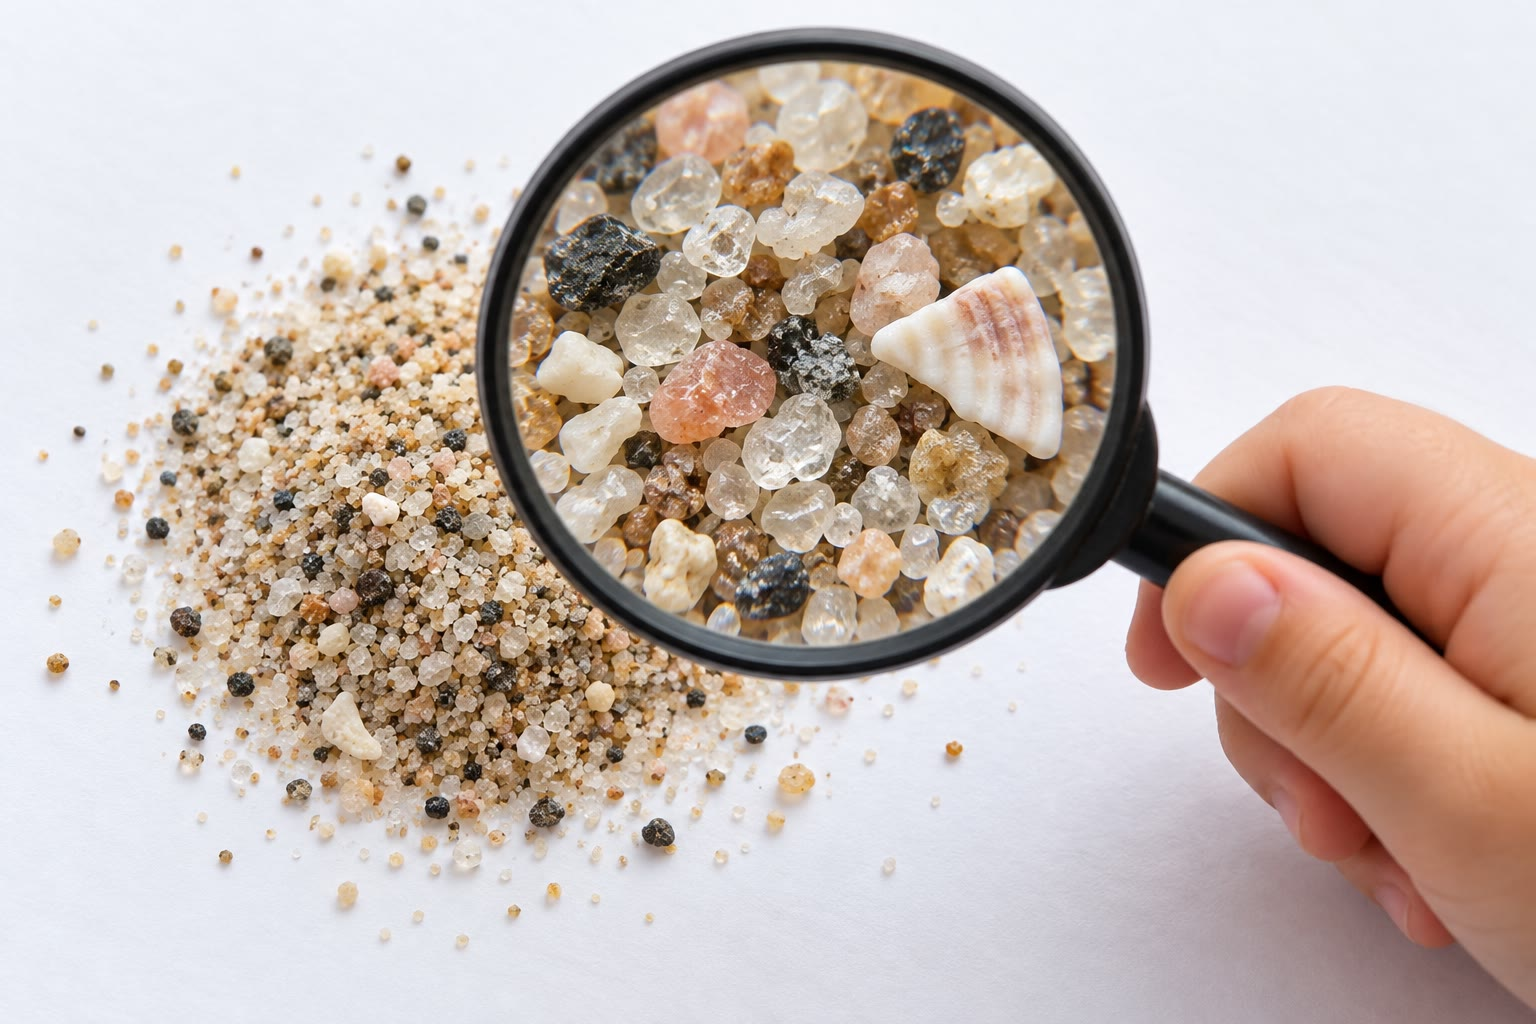
\includegraphics[width=0.55\linewidth]{images/book1/ai/g3-sand-magnifier.jpg}

{\small \omterm{def:g3:stones-pebbles-sand:sand}{Arena} de playa vista con una lupa: granitos diminutos de \omterm{def:g3:stones-pebbles-sand:rock}{roca} y
trocitos de concha.}
\end{omfigure}

\begin{method}[Clasificar la roca rota por tamaños]\label{met:g3:stones-pebbles-sand:sort}
Para nombrar un trozo de \omterm{def:g3:stones-pebbles-sand:rock}{roca} rota, fíjate en su tamaño:
\begin{enumerate}
  \item si no ves los granos, ni siquiera de cerca, es \omterm{def:g3:stones-pebbles-sand:sand}{barro};
  \item si ves cada grano, pero cada uno mide menos de 2 milímetros (el
        grosor de una moneda), es \omterm{def:g3:stones-pebbles-sand:sand}{arena};
  \item si los trozos son más grandes, pero puedes sostener uno en la mano,
        son \omterm{def:g3:stones-pebbles-sand:pebble}{grava} y \omterm{def:g3:stones-pebbles-sand:pebble}{cantos};
  \item si un trozo pesa demasiado para levantarlo, es un bloque.
\end{enumerate}
\end{method}

\begin{example}[¿Dónde encontramos cada tamaño?]\label{ex:g3:stones-pebbles-sand:where}
El agua rápida puede llevar piedras grandes; el agua lenta las deja caer y
solo lleva granos pequeños. Por eso los bloques y las piedras afiladas
están en los arroyos empinados de \omterm{def:g1:landscapes-around-us:landform}{montaña}; los \omterm{def:g3:stones-pebbles-sand:pebble}{cantos} y la \omterm{def:g3:stones-pebbles-sand:pebble}{grava}, en las
orillas del \omterm{def:g1:landscapes-around-us:water}{río} en el \omterm{def:g1:landscapes-around-us:landform}{valle}; la \omterm{def:g3:stones-pebbles-sand:sand}{arena} se acumula en las playas y en las
curvas tranquilas del \omterm{def:g1:landscapes-around-us:water}{río}; y el \omterm{def:g3:stones-pebbles-sand:sand}{barro} se deposita donde el agua está casi
quieta, en las charcas, los \omterm{def:g1:landscapes-around-us:water}{lagos} y las desembocaduras de los \omterm{def:g1:landscapes-around-us:water}{ríos}.
\end{example}

\section{Rocas duras y rocas blandas}

No todas las \omterm{def:g3:stones-pebbles-sand:rock}{rocas} son igual de duras. Algunas, como el granito, son tan
duras que rayan el vidrio y duran miles de años en un muro. Otras se
desmenuzan en la mano, como la creta, que deja una marca blanca en una
pizarra. Algunas \omterm{def:g3:stones-pebbles-sand:rock}{rocas} están hechas de granos que podemos ver; otras son
lisas y parecen iguales de un lado a otro.

\begin{example}[Comparamos tres rocas]\label{ex:g3:stones-pebbles-sand:three}
El \emph{granito} está moteado de granos rosas, blancos y negros y es muy
duro. La \emph{arenisca} está hecha de granos de \omterm{def:g3:stones-pebbles-sand:sand}{arena} pegados entre sí; si
la frotas con un dedo, a veces suelta unos granos. La \emph{creta} es
blanca, blanda y polvorienta. En un curso posterior aprenderás cómo se
formó cada una.
\end{example}

\begin{omfigure}
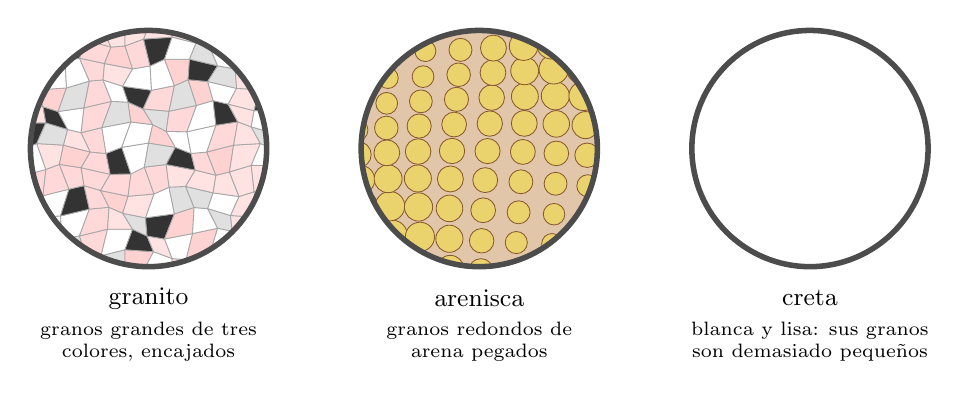
\begin{tikzpicture}[font=\small]
  % three stones seen through a magnifying glass (drawn, not to scale)
  % granite: interlocking grains of three colours
  \begin{scope}
    \clip (0,0) circle (1.5);
    % a jittered lattice: the cells tile the disk with no gap, like the
    % interlocking crystals of granite
    \foreach \i in {-6,...,5} \foreach \j in {-6,...,5} {
      \pgfmathtruncatemacro{\c}{mod(abs(37*\i+17*\j+\i*\j),7)}
      \ifcase\c \def\col{pink!70}\or\def\col{pink!45}\or\def\col{white}\or
        \def\col{black!12}\or\def\col{white}\or\def\col{black!80}\else\def\col{pink!60}\fi
      \fill[\col, draw=black!35, line width=0.3pt]
        ({0.27*\i+0.07*sin(90*\i+131*\j)},{0.27*\j+0.07*cos(77*\i+61*\j)}) --
        ({0.27*(\i+1)+0.07*sin(90*(\i+1)+131*\j)},{0.27*\j+0.07*cos(77*(\i+1)+61*\j)}) --
        ({0.27*(\i+1)+0.07*sin(90*(\i+1)+131*(\j+1))},{0.27*(\j+1)+0.07*cos(77*(\i+1)+61*(\j+1))}) --
        ({0.27*\i+0.07*sin(90*\i+131*(\j+1))},{0.27*(\j+1)+0.07*cos(77*\i+61*(\j+1))}) -- cycle;
    }
  \end{scope}
  \draw[black!70, line width=2pt] (0,0) circle (1.5);
  \node at (0,-1.9) {granito};
  \node[font=\scriptsize, align=center] at (0,-2.45) {granos grandes de tres\\colores, encajados};
  % sandstone: rounded grains touching
  \begin{scope}[xshift=4.2cm]
    \clip (0,0) circle (1.5);
    \fill[brown!45] (-1.6,-1.6) rectangle (1.6,1.6);
    \foreach \x in {-1.5,-1.1,...,1.6} \foreach \y in {-1.5,-1.15,...,1.6}
      \fill[yellow!50!brown!70, draw=brown!70!black, line width=0.3pt]
        ({\x+0.08*sin(97*\x+61*\y)},{\y+0.07*cos(53*\x-89*\y)}) circle ({0.16+0.03*sin(71*\x*\y)});
  \end{scope}
  \draw[black!70, line width=2pt] (4.2,0) circle (1.5);
  \node at (4.2,-1.9) {arenisca};
  \node[font=\scriptsize, align=center] at (4.2,-2.45) {granos redondos de\\arena pegados};
  % chalk: smooth, no grains to see
  \begin{scope}[xshift=8.4cm]
    \fill[white] (0,0) circle (1.5);
  \end{scope}
  \draw[black!70, line width=2pt] (8.4,0) circle (1.5);
  \node at (8.4,-1.9) {creta};
  \node[font=\scriptsize, align=center] at (8.4,-2.45) {blanca y lisa: sus granos\\son demasiado pequeños};
\end{tikzpicture}

{\small Tres \omterm{def:g3:stones-pebbles-sand:rock}{rocas} vistas con una lupa (dibujadas). Los granos del granito y
de la arenisca se ven; la creta parece igual en todas partes.}
\label{fig:g3:stones-pebbles-sand:magnified}
\end{omfigure}

\begin{method}[Mirar una piedra de cerca]\label{met:g3:stones-pebbles-sand:look}
Para describir una piedra, mírala y tócala, sin romperla:
\begin{enumerate}
  \item su color, o sus colores;
  \item su forma: afilada y con esquinas, o redonda y lisa;
  \item sus granos: ¿los ves? ¿son todos iguales o de varios colores?
  \item su tacto: ¿es dura, o tan blanda que deja una marca en el papel?
\end{enumerate}
Escribe lo que ves en una tabla, una fila para cada piedra.
\end{method}

\begin{example}[Una tabla de tres piedras]\label{ex:g3:stones-pebbles-sand:table}
Mía describe tres piedras de una caja del colegio.
\begin{center}\small
\begin{tabular}{llll}
\hline
Piedra & Color & Forma & Granos \\
\hline
A & rosa, blanco y negro & redonda & grandes, de tres colores \\
B & marrón amarillento & afilada & pequeños, todos iguales \\
C & blanco & afilada & no se ven \\
\hline
\end{tabular}
\end{center}
La piedra C también deja una marca blanca en el papel. Según el ejemplo
anterior, la piedra A se parece al granito, la piedra B a la arenisca y la
piedra C a la creta. La piedra A es redonda: el agua la ha hecho rodar
mucho tiempo.
\end{example}

\section{Las piedras con las que construimos}

Desde hace miles de años, la gente construye con la \omterm{def:g3:stones-pebbles-sand:rock}{roca} que tiene a su
alrededor. En los pueblos antiguos de una región, los muros suelen ser
todos del mismo color, porque se construyeron con la piedra de la \omterm{def:g1:landscapes-around-us:landform}{colina}
más cercana.

\begin{definition}[Piedra de construcción]\label{def:g3:stones-pebbles-sand:building-stone}
Una \emph{piedra de construcción}\index{piedra de construccion@piedra de construcción}
es una \omterm{def:g3:stones-pebbles-sand:rock}{roca} que se corta o se labra para construir muros, tejados,
escalones, puentes o pavimentos.
\end{definition}

Cada \omterm{def:g3:stones-pebbles-sand:rock}{roca} sirve para algo. El granito, que es duro, sirve para muros,
escalones y bordillos que duran siglos. Algunas \omterm{def:g3:stones-pebbles-sand:rock}{rocas}, como la pizarra, se
parten en láminas finas y planas: colocadas unas sobre otras, forman
tejados que no dejan pasar la lluvia. La arenisca y la caliza son lo
bastante blandas para cortarlas en bloques bien escuadrados.

\begin{omfigure}
\begin{minipage}[b]{0.49\linewidth}\centering
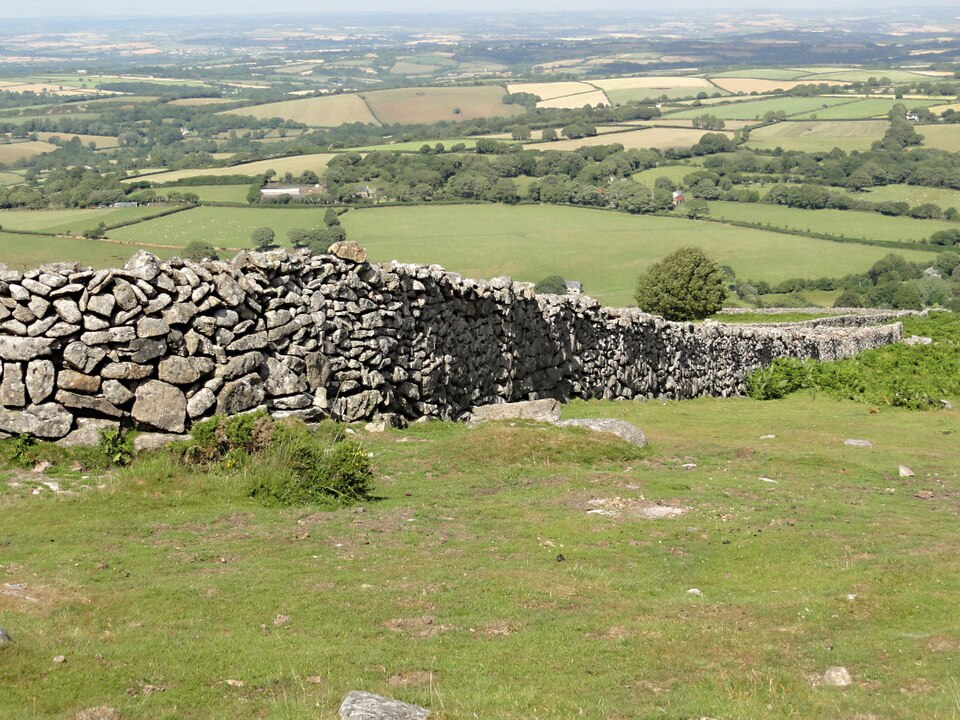
\includegraphics[width=\linewidth]{images/book1/g3-granite-wall.jpg}

{\small Un muro de bloques de granito, construido sin mortero. Fotografía:
Tony Atkin, Geograph (CC BY-SA 2.0).}
\end{minipage}\hfill
\begin{minipage}[b]{0.49\linewidth}\centering
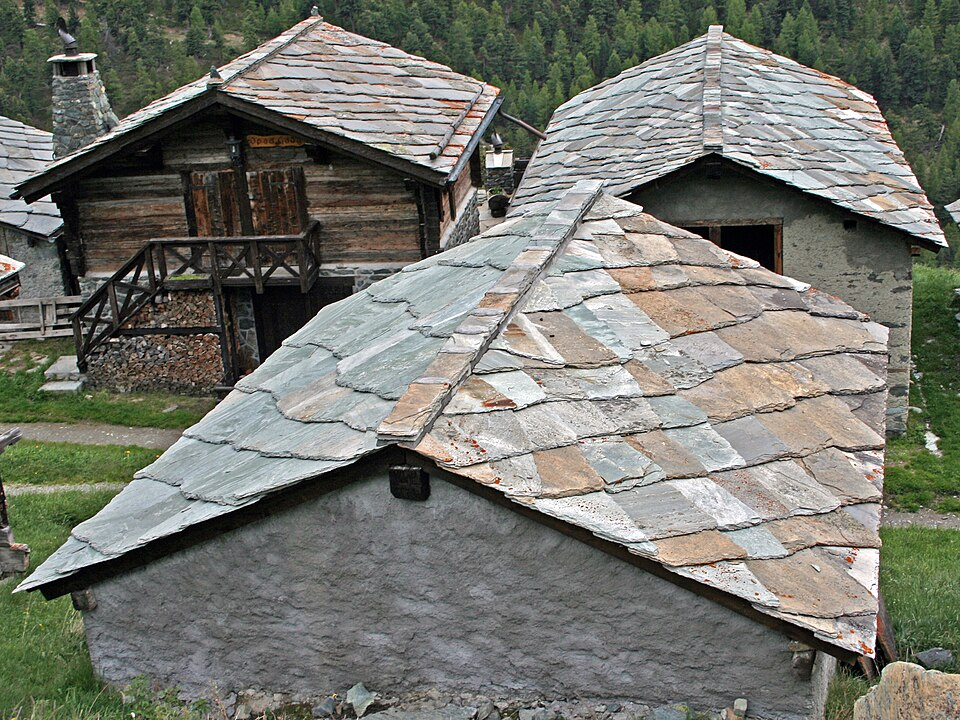
\includegraphics[width=\linewidth]{images/book1/g3-slate-roof.jpg}

{\small Tejados de losas de piedra finas y planas en un pueblo de \omterm{def:g1:landscapes-around-us:landform}{montaña}
de Suiza. Fotografía: Michael C. Rygel (CC BY-SA 3.0).}
\end{minipage}
\end{omfigure}

\begin{omfigure}
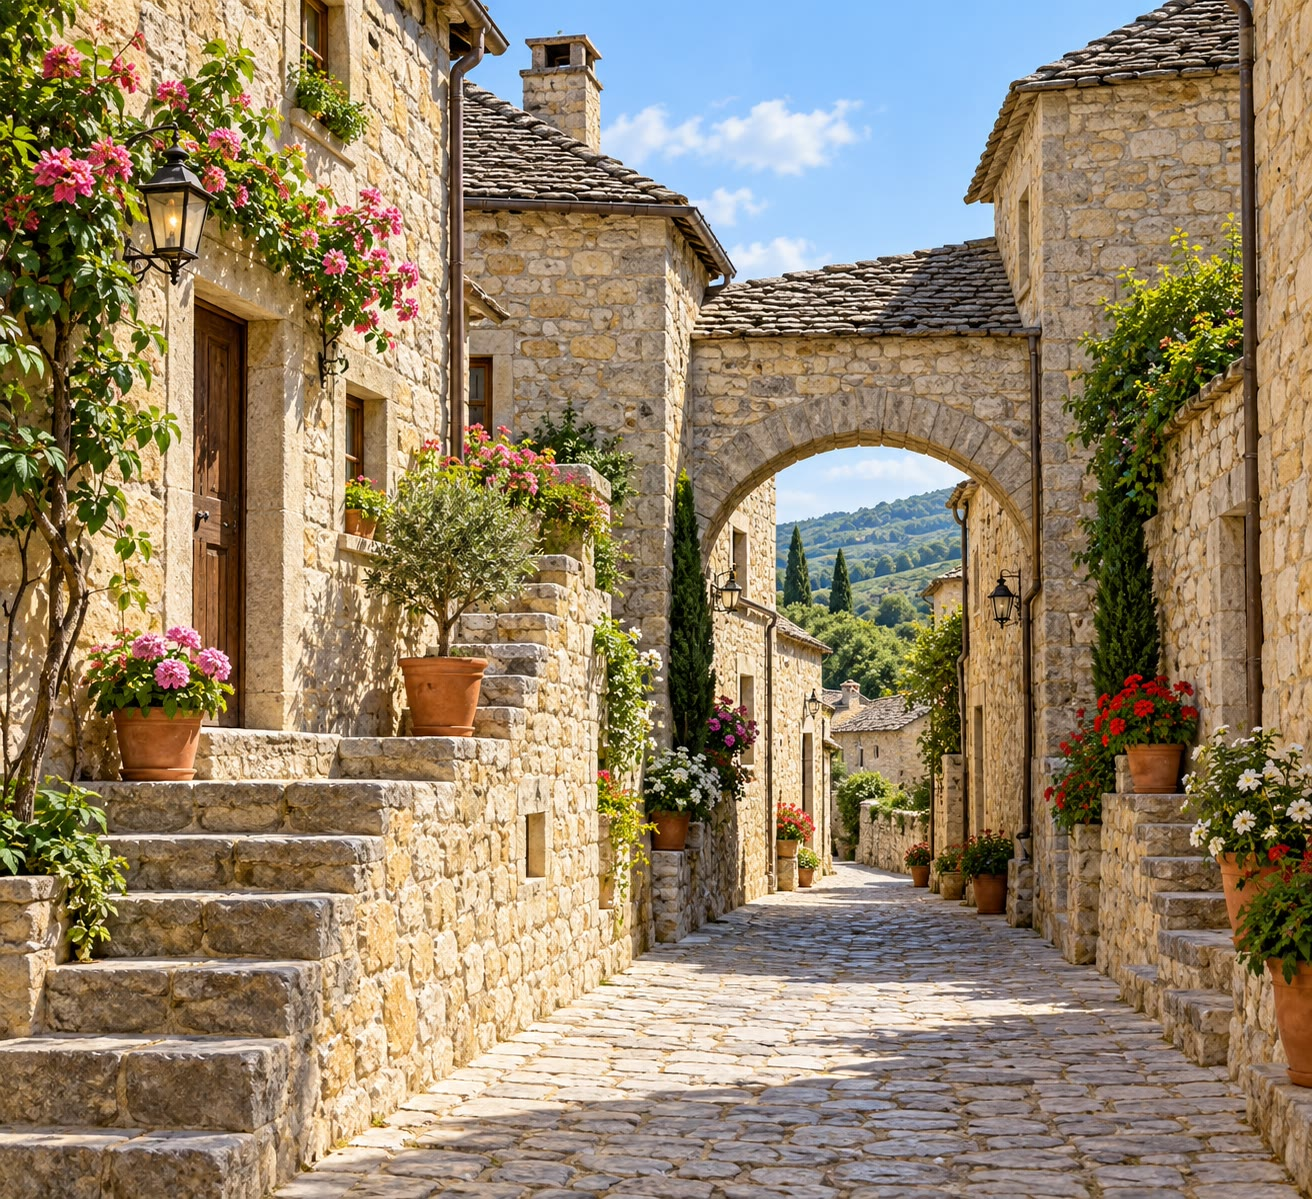
\includegraphics[width=0.6\linewidth]{images/book1/ai/g3-stone-village.jpg}

{\small Un pueblo antiguo construido por completo con la piedra de la
\omterm{def:g1:landscapes-around-us:landform}{colina} cercana.}
\end{omfigure}

Hoy también construimos con ladrillos, hormigón y vidrio. Pero un ladrillo
está hecho de arcilla cocida, el hormigón de \omterm{def:g3:stones-pebbles-sand:sand}{arena}, \omterm{def:g3:stones-pebbles-sand:pebble}{grava} y cemento, y el
vidrio se fabrica con \omterm{def:g3:stones-pebbles-sand:sand}{arena}: todos ellos vienen también de las \omterm{def:g3:stones-pebbles-sand:rock}{rocas} de la
Tierra.

\section{Ejercicios}

\begin{exercise}[$\star$]\label{exo:g3:stones-pebbles-sand:1}
¿Qué es el \omterm{def:g3:stones-pebbles-sand:rock}{lecho rocoso}? ¿Dónde podemos verlo sin cavar?
\end{exercise}

\begin{exercise}[$\star$]\label{exo:g3:stones-pebbles-sand:2}
Ordena por tamaño, del más pequeño al más grande: \omterm{def:g3:stones-pebbles-sand:pebble}{canto rodado}, \omterm{def:g3:stones-pebbles-sand:sand}{barro},
bloque, \omterm{def:g3:stones-pebbles-sand:sand}{arena}.
\end{exercise}

\begin{exercise}[$\star$]\label{exo:g3:stones-pebbles-sand:3}
Un grano mide 1 milímetro de diámetro. ¿Es \omterm{def:g3:stones-pebbles-sand:sand}{arena} o \omterm{def:g3:stones-pebbles-sand:pebble}{grava}? Otro grano mide
3 milímetros: ¿\omterm{def:g3:stones-pebbles-sand:sand}{arena} o \omterm{def:g3:stones-pebbles-sand:pebble}{grava}?
\end{exercise}

\begin{exercise}[$\star$]\label{exo:g3:stones-pebbles-sand:4}
¿Natural o hecho por la gente? Un \omterm{def:g3:stones-pebbles-sand:pebble}{canto rodado}; un ladrillo; un bloque de
granito; una lámina de vidrio; la \omterm{def:g3:stones-pebbles-sand:sand}{arena} de una playa.
\end{exercise}

\begin{exercise}[$\star$]\label{exo:g3:stones-pebbles-sand:5}
¿Por qué un \omterm{def:g3:stones-pebbles-sand:pebble}{canto} de \omterm{def:g1:landscapes-around-us:water}{río} no tiene esquinas afiladas?
\end{exercise}

\begin{exercise}[$\star$]\label{exo:g3:stones-pebbles-sand:6}
Nombra dos \omterm{def:g3:stones-pebbles-sand:building-stone}{piedras de construcción} y di para qué sirve cada una en las
fotografías de este capítulo.
\end{exercise}

\begin{exercise}[$\star\star$]\label{exo:g3:stones-pebbles-sand:7}
Tom encuentra dos piedras de la misma \omterm{def:g3:stones-pebbles-sand:rock}{roca}: una es afilada y la otra es
redonda. ¿Cuál ha viajado más lejos? Explícalo.
\end{exercise}

\begin{exercise}[$\star\star$]\label{exo:g3:stones-pebbles-sand:8}
En el dibujo de los tamaños de grano, ¿cuántos centímetros mide el \omterm{def:g3:stones-pebbles-sand:pebble}{canto} más
grande? ¿Cuántos granos de \omterm{def:g3:stones-pebbles-sand:sand}{arena} de 2 milímetros cabrían uno al lado del
otro a lo largo de 1 centímetro?
\end{exercise}

\begin{exercise}[$\star\star$]\label{exo:g3:stones-pebbles-sand:9}
¿Dónde esperarías encontrar \omterm{def:g3:stones-pebbles-sand:sand}{barro}: en un arroyo de \omterm{def:g1:landscapes-around-us:landform}{montaña} rápido o en una
charca tranquila? ¿Por qué?
\end{exercise}

\begin{exercise}[$\star\star$]\label{exo:g3:stones-pebbles-sand:10}
Los ladrillos, el hormigón y el vidrio los fabrica la gente. ¿Por qué
podemos decir, aun así, que vienen de las \omterm{def:g3:stones-pebbles-sand:rock}{rocas} de la Tierra?
\end{exercise}
